% Created 2018-05-12 Sat 19:23
\documentclass[9pt, b5paper]{article}
\usepackage{fontspec}
\usepackage{graphicx}
\usepackage{xcolor}
\usepackage{xeCJK}
\setCJKmainfont[BoldFont = Songti SC Bold, ItalicFont = STFangsong]{Songti SC}
\setCJKsansfont{STHeiti}
\setCJKmonofont{STFangsong}
\usepackage{multirow}
\usepackage{multicol}
\usepackage{float}
\usepackage{textcomp}
\usepackage{geometry}
\geometry{left=0.1cm,right=0.1cm,top=0.1cm,bottom=0.1cm}
\usepackage{algorithm}
\usepackage{algorithmic}
\usepackage{latexsym}
\usepackage{natbib}
\usepackage{listings}
\usepackage{minted}
\usepackage[xetex,colorlinks=true,CJKbookmarks=true,linkcolor=blue,urlcolor=blue,menucolor=blue]{hyperref}
\author{deepwaterooo}
\date{\today}
\title{AR First App}
\hypersetup{
  pdfkeywords={},
  pdfsubject={},
  pdfcreator={Emacs 25.3.1 (Org mode 8.2.7c)}}
\begin{document}

\maketitle
\tableofcontents


\section{Udpates}
\label{sec-1}
\begin{itemize}
\item I consider so far all visible/noticable bugs has been cleared out, and temporatorily leave the project this way for a while. .apk file is included in the repository if any one want to try install and run. 

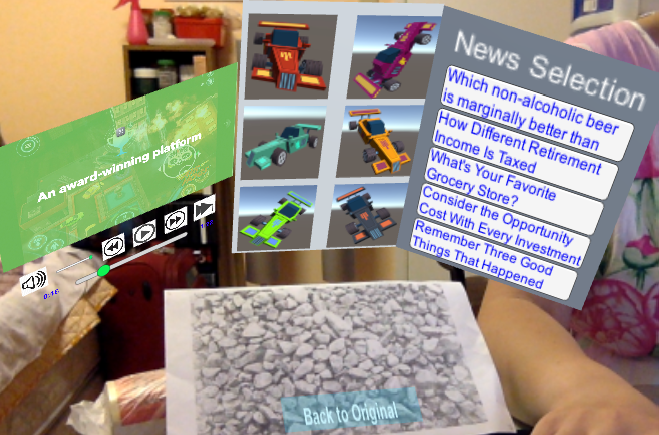
\includegraphics[width=.9\linewidth]{./pic/another.png}
\item Clean up bugs: 
\begin{itemize}
\item VideoPlayer control when lost track: 
\begin{itemize}
\item Customize TrackableEventHandler so that if videoplayer is playing, when lost track, pause; when get back to be reconnected, continue playing
\end{itemize}
\item fastfard: fast backward is allowed during both playing and pause, but fast forward is only allow during playing.
\end{itemize}
\item LeanScale: under control for separating scaling videoplayer from scaling car models.
\item Try to clean all bugs that get noticed: 
\begin{itemize}
\item adjust the video plain size/ratio to display video properly
\item next clip button resulted crashes
\item volume slider and video slider works perfectly just as videoplayer section user interaction GUI design and implementation are perfect right now \textasciitilde{}!
\item Car selection section removed left over car models when user interacts other sections.
\item news selection section added possiblity to surfe and view original news, as well as some button kept display new texts.
\item Will make at least another commit to summarize: include android phone screen recorded videos, and NewsAPI small part video to fetch news form online.
\end{itemize}
\item All major functionalities are finished. One screen shot was attached. 

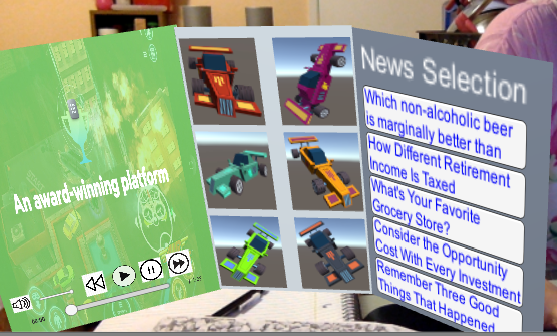
\includegraphics[width=.9\linewidth]{./pic/one.png}
\begin{itemize}
\item Will continueously smooth the project a little bit more (maybe a couple of days) to see if there is anything else that I can do for it.
\end{itemize}
\item video play part user interaction are completely finished. Will fill in the rest necessary components for news selection section to complete.
\item Play Pause function works, interface needs to be improved.
\item will make video user interaction work first, then modify others. 
\begin{itemize}
\item video works only without user interaction (play, pause)
\item car selection secton works
\item news selection basically works, hard coded five news, display in a new plain
\item Others: news API call works, NewsAPI client library works
\end{itemize}
\end{itemize}
% Emacs 25.3.1 (Org mode 8.2.7c)
\end{document}